\documentclass[10pt]{paper}
\usepackage[a4paper, total={6in, 9in}, bottom = 1in]{geometry}
\usepackage[utf8]{inputenc}
\usepackage[slovak]{babel}
\usepackage{fancyhdr}
\usepackage{mathtools}
\usepackage{pgfplots}
\usepackage{wrapfig}
\usepackage{amsmath}
\usepackage{algpseudocode}
\usepackage{paracol}
\usepackage{enumitem}
\newcommand{\name}{Katarína Kejstová 433820, Viktória Vozárová 433334}
\newcommand{\datum}{Projekt IV109}
\pagestyle{fancy}
\fancyhf{}
\lhead{\name}
\rhead{\datum}
\setlength\parindent{0pt}
\begin{document}

\begin{titlepage}
\begin{center}
  \bfseries
  \huge Záverečná správa
  \vskip.2in
  \textsc{\LARGE projektu IV109 }
  \vskip1in
  \emph{\huge Robot - zbieranie pokladu}
\end{center}

\vskip3in

\begin{minipage}{.45\textwidth}
  \begin{flushleft}
    \bfseries\large Prednášajúci:\par \emph{doc. Mgr. Radek Pelánek, Ph.D.}
  \end{flushleft}
\end{minipage}
\hskip.15\textwidth
\begin{minipage}{.40\textwidth}
  \begin{flushleft}
    \bfseries\large Študenti:\par \emph{Katarína Kejstová} 433820 \par \emph{Viktória Vozárová} 433334
  \end{flushleft}
\end{minipage}

\vskip1.3in

\centering
\bfseries
\Large Jarný semester 2016
\end{titlepage}

\section{Zadanie projektu}

\textit{Variace na příklad zmíněný na přednášce. Robot se pohybuje v čtvercové mřížce, na některých polích jsou poklady, které má posbírat, případně zdi, díry, a pod. Vytvořte genetický algoritmus, který bude vytvářet navigační kód pro robota (tak aby posbíral co nejvíce pokladu).}

\section{Genetické algoritmy}
 
Genetické algoritmy sú vo všeobecnosti heuristické postupy, aplikujúce princípy z evolučnej biológie. Často sú využívané na riešenia zložitých problémov, pretože sú schopné vytvoriť netriviálne (náhodné) riešenia. Než začneme s popisom nášho riešenia problému, je potrebné definovať niektoré pojmy spájajúce sa s genetickými algoritmami a ich aplikáciou v praxi.\\

\textbf{Chromozóm}

V aplikácii genetických algoritmov je chromozóm chápaný ako reťazec, resp. postupnosť symbolov, reprezentujúci jedinca s výslednými vlastnosťami. Každá vlastnosť nejako popisuje riešenie a preto reťazec chápeme ako riešenie.\\

\textbf{Gén}

Je základnou časťou chromozómómu. Jeden gén popisuje jednu vlastnosť. Často je reprezentovaný jedným symbolom chromozómu - reťazca, avšak môže byť tvorený aj spojením symbolov - podreťazec.\\

\textbf{Populácia}

Populáciou rozumieme skupinu reťazcov, a teda potencionálnych riešení. Nad touto skupinou aplikujeme jednu iteráciu genetického algorimu, výstupom je nová populácia. Veľkosť populácie môže byť premenlivá, v našej aplikácii však pre jeden beh algoritmu udržiavame populáciu konštantnú.\\

\textbf{Fitness funkcia}

Táto funkcia priradí každému chromozómu, a teda riešeniu hodnotu, vypovedajúcu o jeho úspešnosti. Fitness funkcia pomáha optimalizovať riešenie na základe snahy získať chromozóm s maximálnym ohodnotením. Táto funkcia by preto mala byť vhodne definovaná.

V našej aplikácii sú použité a porovnané rôzne fitness funkcie a ich vplyv na výsledné riešenie (úspešnosť robota). Každá funkcia zároveň potrebuje inak vyladené parametre, by ktorých dáva najlepšie výsledky. Tento fakt tiež zohľadníme v našej analýze.\\

\textbf{Kríženie}

Kríženie využívame pri procese vzniku novej generácie potomkov. Vďaka kríženiu vznikajú nové, odlišné jedince. V kontexte genetických algoritmov tým rozumieme vytvorenie nového reťazca kombináciou dvoch reťazcov z aktuálnej populácie. 

Pri krížení zvolíme náhodný bod na chromozóme, $i$, a potom skrížením dvoch reťazcov $A,B$ vznikne potomkom reťazec $C = A[1..i] + B[i+1..n]$, kde $n$ je koniec reťazca $B$.\\

\textbf{Mutácia}

Mutácia je proces náhodnej modifikácie určitého génu chromozómu z množiny prístupných vlastností. Zmena génu sa uskutoční s určitou dopredu danou, a často pomerne malou, pravdepodobnosťou. To zaručí objavovanie nových riešení, ku ktorým by sme sa inak nedostali. Zabraňuje uviaznutiu v lokálnom optime. Mutácia doplňuje operáciu kríženia, a teda vytvárania novej generácie potomkov. Môže byť vynechaná.

\newpage

\section{Analýza problému}

Prostredie, v ktorom sa robot pohybuje, je reprezentované ohraničenou mapou, na ktorej je statický počet pokladov a nejaké rozmiestnené prekážky. Uvažujeme dve rôzne mapy líšiace sa obtiažnosťou (množstvom prekážok). Všetky roboty začínajú na dopredu danej počiatočnej pozícii.

V kontexte nášho problému pod pojmom \textbf{gén} chápeme symbol z množiny \{$L, R, U, D$\}, reprezentujúci pohyb po mape (doľava, doprava, hore, dole). \textbf{Chromozómom} je reťazec symbolov pohybu, takže určuje celú cestu robota na mape. Dĺžka reťazca závisí od veľkosti mapy. Pri príliš krátkej ceste nemá robot šancu pozbierať dostatočné množstvo pokladu, pri príliš dlhom robí zbytočne veľa krokov navyše a tým stráca na kvalite. 

Pri analýze sme uvažovali rôzne \textbf{fitness funkcie} líšiace sa v ohodnotení pohybu. Rozlišujeme, kedy robot nájde poklad, narazí na stenu alebo ani jedno z toho. V prípade, že robot narazí na stenu, ostane stáť na mieste.

Kríženie aj mutácie prebiehajú vždy s dopredu danou pravdepodonosťou na celý beh genetického algorimtu.

\section{Aplikácia genetického algoritmu}
Daný problém riešime oddelene vzhľadom na dve rôzne mapy (obrázok 1, obrázok 2), s ktorými budeme pracovať pri ďalších analýzach. Počet pokladov na každej mape je $10$, veľkosť každej mapy je $10$x$10$. Rovnako je nemenná počiatočná poloha robota.

\begin{center}
\columnratio{0.5,0.5}
\begin{paracol}{2}
\setlength{\columnseprule}{0pt}
\setlength{\columnsep}{0em}
\begin{leftcolumn}
	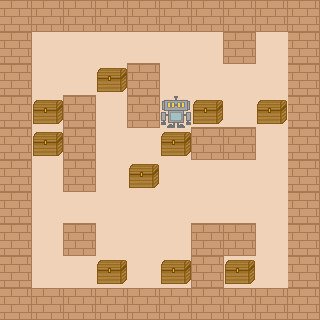
\includegraphics[scale=0.5]{simple_map.png} \\
	Obrázok 1: jednoduchá mapa
\end{leftcolumn}

\begin{rightcolumn}
	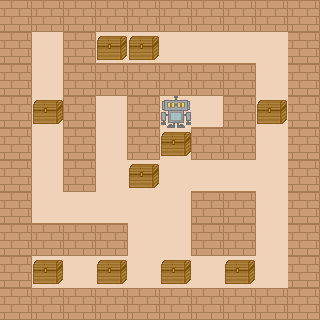
\includegraphics[scale=0.5]{complicated_map.png} \\
	Obrázok 2: komplikovaná mapa
\end{rightcolumn}
\end{paracol}
\end{center}

V ďalších obrázkoch pohyb robota na mape reprezentujeme červenou farbou tak, že opakovaný priechod určitým miestom sposobí silnejšie červené zafarbenie. Tým ukážeme, kadiaľ robot prešiel, a zároveň kde robil zbytočné kroky navyše.

Pri testovaní algoritmu budeme uvažovať nasledujúce parametre:

\begin{tabular}{ll}
\hline
\textsc{Population Size} & určuje veľkosť populácie po celú dobu výpočtu \\ 
\textsc{Generations} & počet generácii \\
\textsc{Crossover}  & pravdepodobnosť kríženia  \\
\textsc{Mutation}  &  pravdepodobnosť mutácie génov  \\
\textsc{MinBound \& MaxBound}  &  minimálna a maximálna dĺžka trasy robota \\ \hline
\end{tabular}

\section{Analýza algoritmu pri rôznych parametroch}

Pre jednoduchosť sme počas analýzy nemenili parameter veľkosti populácie, pre všetky behy platí \textsc{Population Size} = 100. Ďalej nemeníme počiatočnú množinu riešení, ktorá je tvorená náhodnými reťazcami dlhými $20$ až $80$ symbolov. Definujeme dve rôzne fitness funkcie a pre každú identifikujeme, pri akých pravdepodobnostiach kríženia a mutácie funguje najlepšie. Následne ich porovnáme navzájom a zhodnotíme, ktorá je efektívnejšia a pokúsime sa zdôvodniť prečo.

\subsection{Fitness funkcie}
\subsubsection{Funkcia s negatívnym ohodnotením}
Fitness funkcia sa pri jednotlivých pohyboch správa nasledovne:
\begin{itemize}[noitemsep]
\item Ak robot nájde poklad, získa 20 bodov.
\item Ak narazí na stenu, stratí 5 bodov.
\item Inak robot získa 1 bod.
\end{itemize}
Robota odmeníme ak nájde poklad, a potrestáme, ak narazí do steny. Zároveň ho motivujeme objavovať nové časti mapy tým, že ho odmeníme za každý krok. Avšak pri veľmi malom pomere odmeny za poklad a za chodenie táto stratégia generuje dlhé riešenia, ktoré však nájdu malý počet pokladov.

Pre danú funkciu sme vyskúšali, ako dobré riešenia vďaka nej natrénujeme pri rôznych parametroch. Konkrétne sme menily parametre pravdepodobnosti kríženia a mutácií. Veľkosť populácia bola vo všektých behoch 100, počet generácií 1000. Pre každú kombináciu sme spustili algoritmus 10-krát a výsledky spriemerovali. Pozorovali sme najlepšieho (best) a najhoršieho (worst) jedinca poslednej generácie a priemerné ohodnotenie jedincov v poslednej generácii (mean). Získané údaje sú v nasledujúcich tabulkách.

\begin{center}
\columnratio{0.5,0.5}
\begin{paracol}{2}
\setlength{\columnseprule}{0pt}
\setlength{\columnsep}{0em}
\begin{leftcolumn}
	Tabulka 1: jednoduchá mapa
	
	
\begin{tabular}{|ll|lll|}
\hline
 \textsc{Cross} & \textsc{Mut}  & best & mean & worst \\ \hline
0.8 & 0.05 & 196.0 & 160.914 & -2.8 \\
0.8 & 0.1 & 184.7 & 146.175 & -10.0 \\
0.8 & 0.2 & 173.4 & 135.798 & -49.7 \\
\hline
0.7 & 0.05 & 201.7 & 146.792 & 1.1 \\
0.7 & 0.1 & 184.5 & 128.331 & -15.8 \\
0.7 & 0.2 & 166.1 & 112.903 & -33.5 \\
\hline
0.6 & 0.05 & 199.3 & 131.23 & 2.7 \\
0.6 & 0.1 & 183.0 & 110.232 & -28.6 \\
0.6 & 0.2 & 174.3 & 98.907 & -43.0 \\
		
\hline
\end{tabular}
\end{leftcolumn}

\begin{rightcolumn}

	Tabulka 2: komplikovaná mapa
\begin{tabular}{|ll|lll|}
\hline
 \textsc{Cross} & \textsc{Mut}  & best & mean & worst \\ \hline

0.8 & 0.05 & 153.3 & 124.477 & -82.3 \\
0.8 & 0.1 & 148.5 & 119.74 & -88.6 \\
0.8 & 0.2 & 140.1 & 107.027 & -97.3\\
\hline
0.7 & 0.05 & 165.4 & 115.37 & -70.2 \\
0.7 & 0.1 & 152.1 & 97.868 & -126.6 \\
0.7 & 0.2 & 135.5 & 90.352 & -103.6 \\
\hline
0.6 & 0.05 & 162.0 & 98.587 & -94.4 \\
0.6 & 0.1 & 161.9 & 92.911 & -119.7 \\
0.6 & 0.2 & 141.8 & 76.222 & -118.7 \\
		
\hline
\end{tabular}	

\end{rightcolumn}
\end{paracol}
\end{center}

Pre každú pravdepodobnosť kríženia je vhodné zvoliť čo najmenšiu pravdepodobnosť mutácie. Neskúšali sme algoritmus bez mutácií, takže nevieme, aká je hranica, pri ktorej by sa jeho výkon prestal zlepšovať. Pre pravdepodobnosť mutácie 0.05 nevieme vybrať najlepšiu pravdepodobnosť kríženia, pretože všetky výsledky sú veľmi podobné. Môžme tvrdiť, že zmena pravdepodobnosti kríženia v intervale 0.6 až 0.8 výkon algoritmu viditeľne neovplyvňuje. Pozorujeme, že na komplikovanej mape algoritmus funguje o niečo horšie ako na jednoduchej. 

V nasledujúcich tabuľkách uvádzame skutočný počet objavených pokladov pre ekvivaletný beh programu.
\begin{center}
\columnratio{0.5,0.5}
\begin{paracol}{2}
\setlength{\columnseprule}{0pt}
\setlength{\columnsep}{0em}
\begin{leftcolumn}
	Tabulka 3: jednoduchá mapa
	
	
\begin{tabular}{|ll|lll|}
\hline
 \textsc{Cross} & \textsc{Mut}  & best & mean & worst \\ \hline
0.8 & 0.05 & 7.5 & 6.114 & 2.2 \\
0.8 & 0.1 & 7.4 & 6.112 & 1.5 \\
0.8 & 0.2 & 7.0 & 5.994 & 1.7 \\
\hline
0.7 & 0.05 & 8.0 & 6.121 & 1.7 \\
0.7 & 0.1 & 7.8 & 5.88 & 1.6 \\
0.7 & 0.2 & 7.2 & 5.668 & 1.6 \\
\hline
0.6 & 0.05 & 7.8 & 5.556 & 1.7 \\
0.6 & 0.1 & 7.3 & 5.118 & 1.3 \\
0.6 & 0.2 & 7.4 & 5.287 & 1.1 \\
		
\hline
\end{tabular}
\end{leftcolumn}

\begin{rightcolumn}

	Tabulka 4: komplikovaná mapa
\begin{tabular}{|ll|lll|}
\hline
 \textsc{Cross} & \textsc{Mut}  & best & mean & worst \\ \hline

0.8 & 0.05 & 5.8 & 5.037 & 1.8 \\
0.8 & 0.1 & 6.0 & 5.304 & 1.6 \\
0.8 & 0.2 & 5.6 & 4.648 & 1.1 \\
\hline
0.7 & 0.05 & 5.8 & 4.887 & 1.3 \\
0.7 & 0.1 & 5.8 & 4.794 & 1.0 \\
0.7 & 0.2 & 5.8 & 4.562 & 1.3 \\
\hline
0.6 & 0.05 & 5.8 & 4.473 & 1.2 \\
0.6 & 0.1 & 6.2 & 4.723 & 1.3 \\
0.6 & 0.2 & 6.2 & 4.709 & 1.1 \\
		
\hline
\end{tabular}	

\end{rightcolumn}
\end{paracol}
\end{center}

 
\begin{center}
  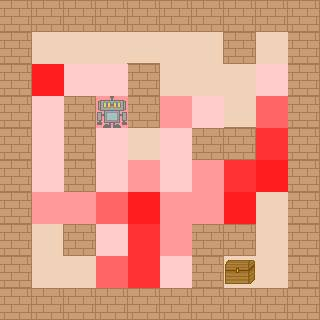
\includegraphics[scale=0.4]{strategy1_simple.png} 
  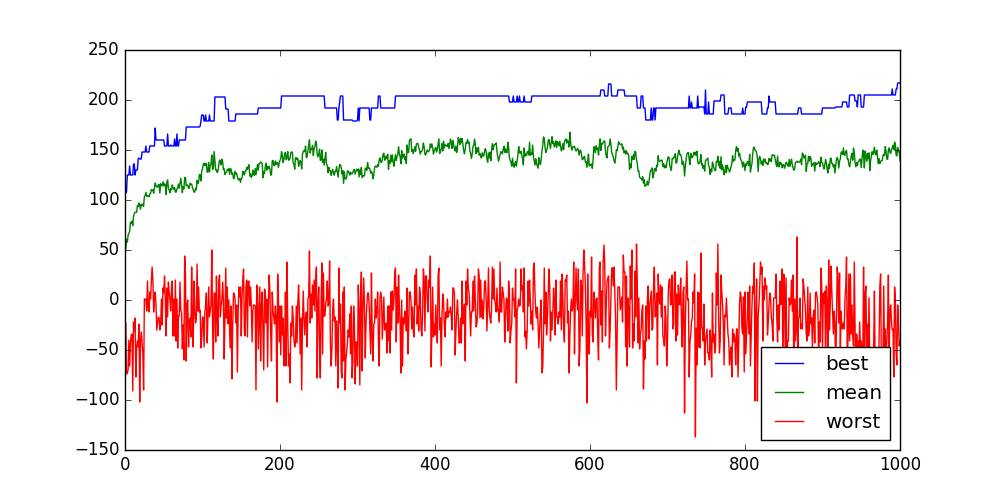
\includegraphics[scale=0.3]{strategy1_simple_graph.png} \\
   Obrázok 3: \textbf{jednoduchá mapa}, vľavo najlepšia cesta, vpravo proces učenia
\end{center}
     
\begin{center}
  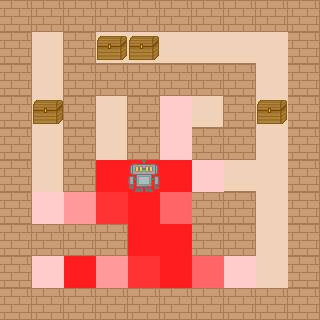
\includegraphics[scale=0.4]{strategy1_complicated.png} 
  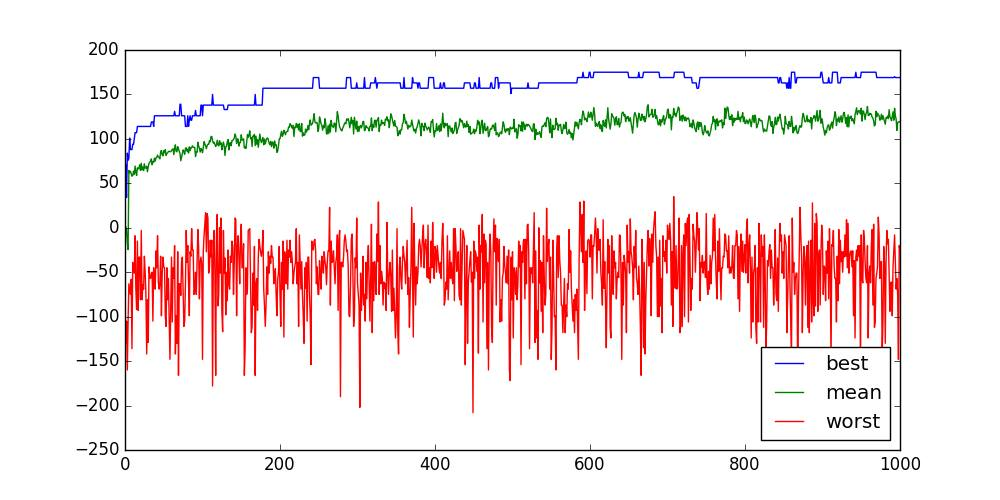
\includegraphics[scale=0.3]{strategy1_complicated_graph.png} \\
   Obrázok 4: \textbf{komplikovaná mapa}, vľavo najlepšia cesta, vpravo proces učenia
\end{center}

\subsubsection{Objektívna funkcia}
Funkciu nazveme objektívnou, pretože zodpovedá presnému počtu pokladov, ktoré robot pozbiera. Funkcia má teda nasledovné správanie:
\begin{itemize}[noitemsep]
\item Ak robot nájde poklad, získa 1 bod.
\item Iný pohyb nemá vplyv na ohodnotenie.
\end{itemize} 

Algoritmus sme opäť spustili 10-krát pre každú kombináciu parametrov, rovnako ako pre predošlä funkciu s nemennou veľkosťou populácie 100 a počtom generácií 1000.


\begin{center}
\columnratio{0.5,0.5}
\begin{paracol}{2}
\setlength{\columnseprule}{0pt}
\setlength{\columnsep}{0em}
\begin{leftcolumn}
	Tabulka 5: jednoduchá mapa	
\begin{tabular}{|ll|lll|}
\hline
 \textsc{Cross} & \textsc{Mut}  & best & mean & worst \\ \hline
0.8 & 0.05 & 9.2 & 7.959 & 3.4 \\
0.8 & 0.1 & 9.4 & 7.451 & 2.5 \\
0.8 & 0.2 & 8.9 & 7.157 & 2.3 \\
\hline
0.7 & 0.05 & 9.1 & 7.171 & 2.9 \\
0.7 & 0.1 & 8.9 & 6.381 & 2.2 \\
0.7 & 0.2 & 8.6 & 6.174 & 2.0 \\
\hline
0.6 & 0.05 & 9.0 & 6.756 & 2.7 \\
0.6 & 0.1 & 8.5 & 5.855 & 2.2 \\
0.6 & 0.2 & 8.2 & 4.995 & 1.6 \\		
\hline
\end{tabular}
\end{leftcolumn}
\begin{rightcolumn}

	Tabulka 6: komplikovaná mapa
\begin{tabular}{|ll|lll|}
\hline
 \textsc{Cross} & \textsc{Mut}  & best & mean & worst \\ \hline

0.8 & 0.05 & 8.3 & 7.313 & 2.3 \\
0.8 & 0.1 & 8.0 & 6.558 & 1.7 \\
0.8 & 0.2 & 7.7 & 6.231 & 1.5\\
\hline
0.7 & 0.05 & 8.2 & 6.82 & 2.4 \\
0.7 & 0.1 & 8.2 & 6.113 & 1.8 \\
0.7 & 0.2 & 7.7 & 5.406 & 1.3 \\
\hline
0.6 & 0.05 & 8.2 & 6.305 & 2.2 \\
0.6 & 0.1 & 7.4 & 5.008 & 1.9 \\
0.6 & 0.2 & 7.2 & 4.526 & 1.2 \\
		
\hline
\end{tabular}		
\end{rightcolumn}
\end{paracol}
\end{center}

Kombinácie parametrov vykazujú podobný trend ako pri predošlej funkcii, a teda nízka pravdepodobnosť mutácie je efektívnejšia ako vysoká. Ak porovnáme najlepšie napočítané hodnoty a zohľadníme aj priemer, možeme povedať, že pravdepodobnosť kríženia 0.8 je v skúmanom rozsahu najefektívnejšia.

\begin{center}
  \vspace{10em}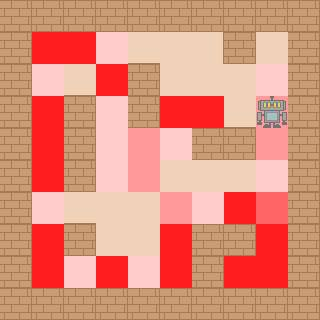
\includegraphics[scale=0.4]{strategy2_simple.png} 
  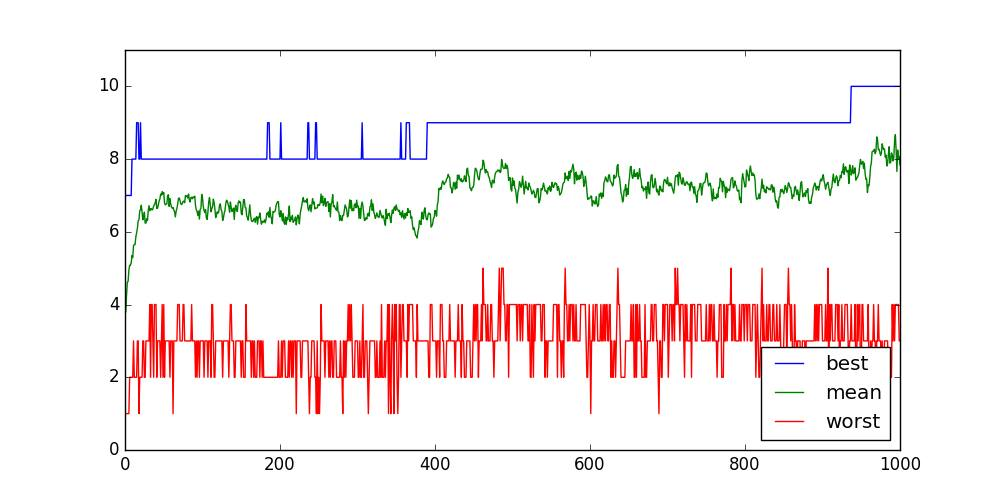
\includegraphics[scale=0.3]{strategy2_simple_graph.png} \\
   Obrázok 5: \textbf{jednoduchá mapa}, vľavo najlepšia cesta, vpravo proces učenia
     \end{center}
     
\begin{center}
  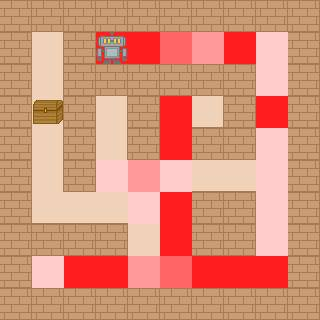
\includegraphics[scale=0.4]{strategy2_complicated.png} 
  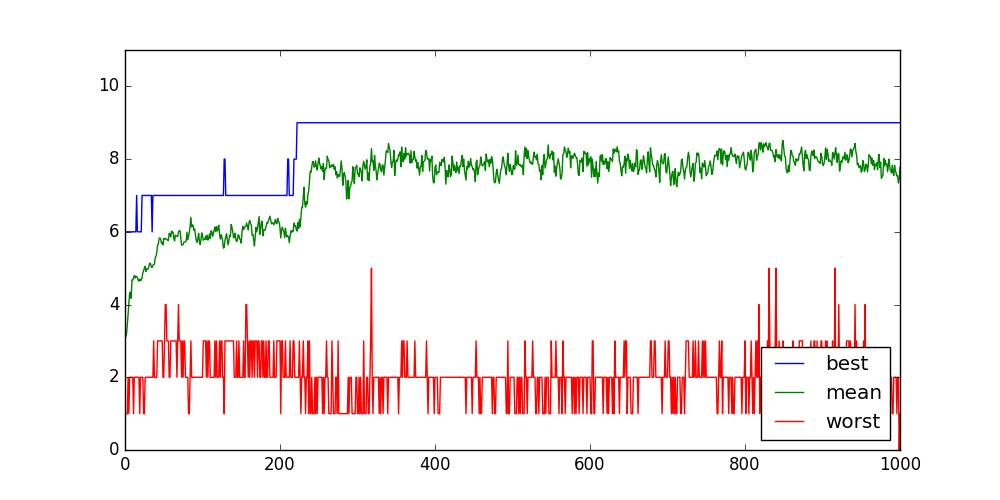
\includegraphics[scale=0.3]{strategy2_complicated_graph.png} \\
   Obrázok 6: \textbf{komplikovaná mapa}, vľavo najlepšia cesta, vpravo proces učenia
     \end{center}
    
\subsection{Porovnanie fitness funkcií}

Porovnáme medzi sebou tabulky 3 a 5 a tabulky 4 a 6. Na prvý pohľad je zjavné, že algoritmus s objektívnou funkciou generuje lepšie riešenia. Efektívnejšia bola teda jednoduchosť, nesnažiť sa robota motivovať aby robil viac krokov alebo nenarážal do stien. Pre dostatočne dobré výsledky stačí každého jedinca ohodnotiť počtom pokladov ktoré nájde. Dôvodom môže byť práve nejednoznačnosť funkcie s negatívnym ohodnotením. Dve rôzne riešenia môžu mať rovnaké ohodnotenie, pričom jedno môže byť značne lepšie ako to druhé (v počte nájdených pokladov).

Skúšali sme aj iné fitness funkcie, ktoré by každy krok ohodnotili zápornou hodnotou. Žiadna z nich neprodukovala dostatočne dobré výsledky, preto ich neuvádzame.

\section{Možnosť rozšírenia problému}

Okrem skúmania rôznych ohodnotení pohybu môžeme pri fitness funkcii uvažovať chovanie pri narazení na stenu. Robot môže ostať stáť, čo je prístup, ktorý sme použili mi, alebo úplne ukončiť vyhodnocovanie svojej cesty. Problém sa dá rozšíriť na väčšie mapy, náhodne generované mapy, mapy bez ohraničenia - pri prejdení cez okraj sa robot objaví na opačnej strane. Môžeme do chromozómu pridať počiatočnú pozíciu robota na mape, ktorú sa algoritmus bude snažiť optimalizovať.

\section{Záver}

Navrhli sme a implementovali riešenie problému podľa štruktúry genetického algoritmu. Identifkovali sme parametre algoritmu a skúmali sme, ako ich zmena vplýva na jeho výkon. Porovnali sme výsledky pre jednotlivé kombinácie a určili najlepšiu možnú kombináciu parametrov pre daný problém. Tým považujeme zadanie za splnené.
\section{Zdroje}

Pri popise a tvorbe genetického algoritmu sme sa inšpirovali uvedenou literatúrou. Zdrojový kód a použité obrázky sú autorská tvorba.\\



Zdrojový kód projektu je uložený v Git repozitári na adrese github.com/Kejsty/iv109{\_}project.


\begin{thebibliography}{9}
\bibitem{theano1}
	Eiben, A.E., Smith, J.E. 
	\textit{Introduction to Evolutionary Computing, Second Edition}. 
	Springer, 2015
	
\bibitem{theano2}
	Shiffman, Daniel.
	\textit{The Nature of Code}. 
	\\(http://www.natureofcode.com/book/chapter-9-the-evolution-of-code)
	
\end{thebibliography}

\end{document}\grid
